%INTRODUCTION PAGE

\chapter{Introduction}

This project emphasizes the application of engineering fundamentals to solve real-world challenges. The primary goal of this initiative is to leverage the synergy between Machine Learning and Web Development to address specific societal or research needs identified through an extensive survey. By converting these needs into a well-defined technical problem, the project strives to develop a functional working model that is not only innovative but also aligned with Sustainable Development Goals (SDGs). This introductory chapter provides the foundational context for the study, detailing the background, motivation, and technical objectives that guided the development and implementation of the proposed solution.

\section{Background}

Briefly describe the evolution of Web Development and its transition from static pages to intelligent, data-driven platforms. 

Introduce Machine Learning as the core logic that enables the system to learn from data and make predictions or decisions.

Explain the synergy between the two: why a web interface is the best delivery mechanism for making an ML model accessible to end-users.

 That is clustering of the nearest approximate value. the 42\% who reported no physical or chronic conditions as shown in Figure \ref{fig:Prevalence}.  public health concerns  \cite{b2}.

\begin{figure}[h]
	\centering
	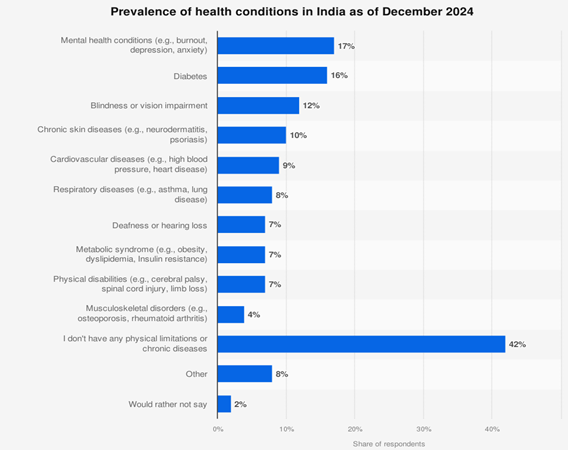
\includegraphics[width=\textwidth]{prevalence.png}
	\caption{Prevalence of health conditions in India as of December 2024 \cite{b2}}
	\label{fig:Prevalence}
\end{figure}

\section{Motivation}
Here, you explain the "Why" behind your project choice.
Detail the specific societal or research needs you discovered during your initial survey.

Discuss the current challenges or pain points faced by the target audience.

Mention your desire to apply engineering fundamentals to solve a real-world problem rather than a purely theoretical one.
\begin{itemize}
	\item Time taken to hire a person. 
	\item Confusion of selecting whom to select.
	\item To improve the tedious process.	
\end{itemize}

\section{Problem Definition}

This is a precise, technical translation of the motivation.
Statement of Need: Summarize the gap identified in Section .

Technical Problem: Convert that need into a technical challenge (e.g., "Designing a robust CNN-based web application to detect crop diseases with an accuracy of over 90\% in real-time").

Scope: Explicitly state what the project will cover and what it will not, ensuring the project is feasible within the semester timeline.

\section{Aim and Objectives of the project}

\subsection{Aim}

Our aim is to help the HR round go more smoothly and efficiently so that a person’s skill can be predicted beforehand without wasting much of the time of the HR. also to sort the resumes according to the requirements of the organizations. And to take the current CV ranking system to an advanced level.

\subsection{Objectives}

Specific goals, including the development of a functional working model. List the "What" of your project in measurable terms.
\begin{itemize}
	\item Identify and pre-process a domain-specific dataset. 
	\item TDesign and train a specific Machine Learning algorithm.
	\item Develop a functional working model with a user-friendly web interface.
	\item Evaluate the model using standard metrics like accuracy, precision, or cost-effectiveness.	
\end{itemize}

\section{Scope of the Project} 

IT sector has largest recruiting sector. Our proposed system is initially concerned with IT companies and to recruit the right candidate with perfect skills and technical skills. IT recruitment is in bulk so to reduce the manual work and make sure the intake is of the right candidate. It is also applicable for different jobs and profession.

\section{Sustainable Development Goal (SDG) Mapping} 
This is a mandatory requirement for analyzing the impact of your solution.
Identify the Goal: Specify the exact UN SDG number and title (e.g., Goal 3: Good Health and Well-being).

Impact Analysis: Provide a detailed explanation of how your specific ML solution contributes to this goal.

Environmental Context: Briefly discuss the sustainability of your solution—how it uses resources efficiently or promotes environmental welfare.\\\\


\section{Organization of the Report} 
The remainder of this report is organized into five subsequent chapters to provide a comprehensive overview of the project’s lifecycle. Chapter 2 presents a detailed literature survey of existing systems and identifies the research gap that justifies the need for this work. Chapter 3 outlines the methodology, system architecture, and project planning, including the Gantt chart for implementation. Chapter 4 details the core implementation phase, covering dataset pre-processing, Machine Learning model development, and the integration of the web-based interface. Chapter 5 provides a demonstration of the working prototype along with an analysis of experimental results and performance metrics. Finally, Chapter 6 concludes the report by summarizing the project's achievements, individual contributions, and potential directions for future research in line with the goals of life-long learning.
